%%%%%%%%%%%%%%%%%%%%%%% file template.tex %%%%%%%%%%%%%%%%%%%%%%%%%
\RequirePackage{fix-cm}
\documentclass[twocolumn]{svjour3}
\smartqed
\usepackage{graphicx}
\usepackage{url}
\usepackage[hidelinks]{hyperref}
\usepackage{array}
\graphicspath{{imgs/}}
\setlength{\emergencystretch}{2em}
\sloppy

\makeatletter
\def\@maketitle{%
  \newpage
  \normalfont
  \global\@topnum\z@
  \hrule\@height 2mm\@width0\p@
  \if@twocolumn
    \ifnum \col@number=\@ne
      \@maketitle@i
    \else
      \twocolumn[\@maketitle@i]%
    \fi
  \else
    \newpage
    \global\@topnum\z@
    \@maketitle@i
  \fi
}

\def\@maketitle@i{%
  \begin{center}%
    {\LARGE\bfseries \@title \par}%
    \vskip 12pt
    \ifx\@subtitle\@empty
    \else
      {\large\itshape \@subtitle \par}%
      \vskip 12pt
    \fi
    {\normalsize\lineskip .5em%
      \begin{tabular}[t]{c}%
        \@author
      \end{tabular}\par}%
    \vskip 10pt
    {\small \@date \par}%
    \vskip 18pt
  \end{center}%
}
\makeatother

\begin{document}

\title{Langify: A Dialect-Adaptive Architecture for Multilingual Real-Time Speech Translation}
\subtitle{Browser-native orchestration of streaming speech capture, contextual translation, and persistent personalization}

\author{Siddhesh H \and
        Abhishek R \and
        Tanmay P}

\institute{Siddhesh H \at
              \email{ram.sidrhirve@gmail.com}
           \and
           Abhishek R \at
              \email{abhishekrajguru16@gmail.com}
           \and
           Tanmay P \at
              \email{tanmaygpatil@gmail.com}}

\date{Received: 23 April 2026 / Accepted: date}

\maketitle

\begin{abstract}
This paper presents Langify, a multilingual speech translation system that combines browser-side audio capture, a low-latency inference pipeline, and a persistent personalization layer for dialect-aware translation. The system is implemented with a Vue 3 and Vite client, a Node.js and Express orchestration server, Groq-hosted Whisper Large v3 Turbo for speech-to-text, LLaMA 3.3 70B for translation, and Supabase for authentication, session storage, vocabulary memory, and post-session summarization. The principal methodological contribution is a Dialect-Adaptive Intelligence (DAI) framework that injects user vocabulary into transcription, carries recent conversational context into translation, and learns new lexical items over time. Unlike a static translate-only pipeline, Langify supports live interaction, session memory, meeting-mode broadcasting, and confidence-aware alternative generation. Repository analysis indicates a production-oriented design with rate limiting, cookie-based session handling, room-based collaboration through Socket.IO, and asynchronous post-session analytics. The resulting contribution extends beyond multilingual transcription to personalized speech understanding in code-switched and domain-sensitive settings.
\keywords{multilingual speech translation \and real-time systems \and dialect adaptation \and code-switching \and speech-to-text \and contextual machine translation}
\subclass{68T50 \and 68U10 \and 68M14}
\end{abstract}

\section{Introduction}
\label{intro}
Real-time speech translation systems are increasingly expected to operate across code-switched speech, informal dialects, and domain-specific terminology rather than only clean monolingual input. In practice, this requirement creates a systems problem as much as a modeling problem. A usable platform must capture audio continuously in the browser, segment speech at low latency, route each segment through automatic speech recognition (ASR) and semantic translation, persist conversational state, and preserve enough context to improve future translations \cite{RefWhisper,RefLlama,RefCodeSwitch}.

Langify addresses this problem through a browser-native pipeline for multilingual live translation with personalization. Repository analysis reveals a three-part design. First, a Vue.js client records speech through the \texttt{MediaRecorder} API and performs silence-aware chunking. Second, an Express-based orchestration server invokes Groq-hosted \mbox{\texttt{whisper-large-v3-turbo}} for transcription and \mbox{\texttt{llama-3.3-70b-versatile}} for translation. Third, a Supabase-backed persistence layer stores sessions, utterances, user profiles, vocabulary updates, and session summaries. The primary methodological addition is the Dialect-Adaptive Intelligence framework, which serves as a contextual layer over the base inference pipeline.

The project makes four engineering contributions. First, it implements a low-latency multilingual translation path that does not require manual source-language selection. Second, it augments this path with DAI-based prompt construction for vocabulary-aware ASR and context-aware translation. Third, it exposes the resulting stream through a collaborative Meeting Mode built on Socket.IO. Fourth, it grounds the interactive pipeline in persistent storage and post-session learning, allowing the system to improve with repeated use.

The remainder of the paper is organized as follows. Section~\ref{sec:related} positions the work relative to multilingual ASR and contextual translation. Section~\ref{sec:architecture} describes the architecture and runtime data flow. Section~\ref{sec:method} explains the DAI framework and translation methodology. Section~\ref{sec:implementation} summarizes implementation details. Section~\ref{sec:evaluation} discusses evaluation evidence available in the repository and the supplied system figures. Section~\ref{sec:discussion} outlines limitations and threats to validity, followed by concluding remarks in Section~\ref{sec:conclusion}.

\section{Background and related work}
\label{sec:related}
Langify sits at the intersection of multilingual ASR, contextual machine translation, and adaptive user modeling. Transformer-based sequence modeling has enabled strong performance in both speech and text processing \cite{RefTransformer}. Whisper-style encoder-decoder ASR systems provide robust multilingual transcription across noisy inputs \cite{RefWhisper}. Large language models further support translation, paraphrase, and inference over mixed-language utterances, especially when system prompts are shaped by task constraints and structured output requirements \cite{RefLlama,RefPrompting}.

However, repository-level speech products often stop at a stateless cascade: record audio, transcribe it, translate it, and discard the interaction history. Such designs underuse two sources of signal. The first is \emph{user-specific vocabulary}, especially important for regional terms, proper nouns, and code-switched expressions. The second is \emph{short-horizon conversational context}, which helps disambiguate fragmented or elliptical speech. Research on contextual ASR and domain adaptation suggests that prompt-side biasing and lexical injection can improve recognition of rare terms when model retraining is unavailable \cite{RefContextASR}. Similarly, conversational translation benefits from local discourse state and intent modeling \cite{RefContextMT}.

Langify differs from a purely stateless pipeline by adding a persistent DAI framework. This framework does not retrain base models. Instead, it builds a structured context packet from a user profile, a vocabulary map, and recent utterances, then injects this packet into the inference path. The result is a pragmatic systems contribution: personalization through orchestration rather than through custom model fine-tuning.

\section{System architecture}
\label{sec:architecture}
The implemented system follows a layered architecture spanning edge capture, server orchestration, AI inference, and persistence. Figure~\ref{fig:architecture} summarizes this design using the supplied system architecture illustration.

\begin{figure*}
\centering
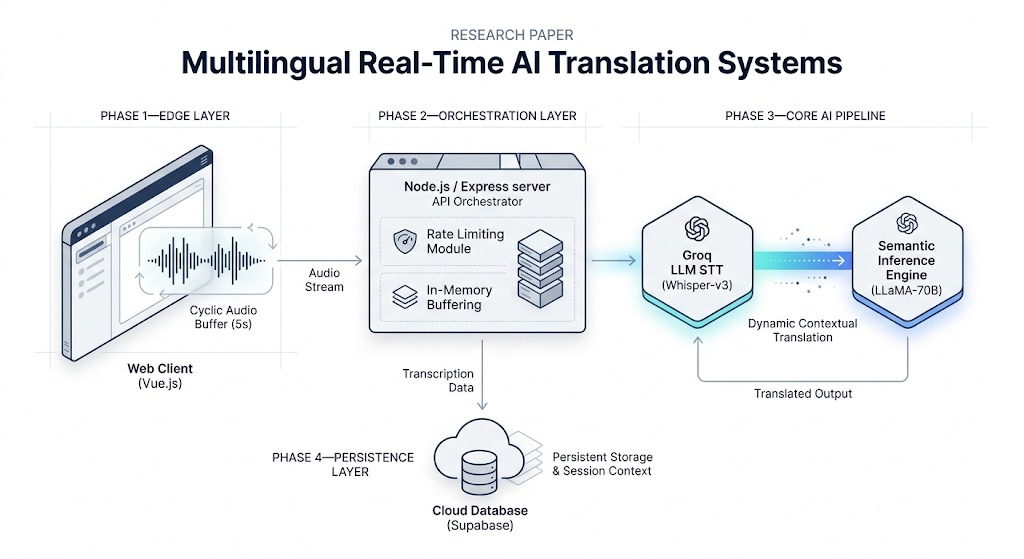
\includegraphics[width=\textwidth]{sys_architecture.jpeg}
\caption{System architecture of Langify. The browser client captures streaming speech, the Express orchestration layer manages request flow and rate limiting, Groq-hosted models perform transcription and translation, and Supabase stores sessions, utterances, and personalization context.}
\label{fig:architecture}
\end{figure*}

At the edge, the Vue 3 client acquires microphone input through \texttt{navigator.mediaDevices.getUserMedia}. The recording subsystem uses \texttt{MediaRecorder} together with an \texttt{AnalyserNode} to segment speech into silence-aware chunks. Rather than using naive fixed windows, the implementation applies a minimum chunk duration of approximately 1.2 seconds, a maximum duration of approximately 6.5 seconds, and an RMS-based silence detector to identify natural speech boundaries. This reduces unnecessary requests during silence while preserving context for translation.

The orchestration layer is implemented in Node.js with Express 5. It provides REST endpoints for authentication, transcription, translation, session lifecycle management, and optional text-to-speech. It also hosts a Socket.IO server for Meeting Mode. Rate limiting is enforced separately for transcription, translation, and authentication endpoints, reflecting an architecture designed for bounded operational cost and resilient public deployment.

The inference layer is a cascade. The first stage sends audio segments to \mbox{\texttt{whisper-large-v3-turbo}} through the Groq SDK, returning verbose JSON transcription metadata when needed. The second stage sends transcribed text to \mbox{\texttt{llama-3.3-70b-versatile}}, which performs translation and, under DAI mode, returns structured JSON containing translated text, detected language, confidence, emotional tone, inferred intent, and low-confidence alternatives.

The persistence layer is implemented through Supabase. The schema includes base entities for \texttt{sessions} and \texttt{utterances}, then extends them with DAI-oriented tables for \texttt{user\_profiles}, \texttt{user\_vocabulary}, and \texttt{session\_summaries}. This design enables both real-time storage and cross-session memory. Authentication is handled through Supabase Auth with server-issued HTTP-only cookies.

\paragraph{Data flow.} The happy path begins when a user starts a live session and selects a target language. The client creates a session record, starts microphone capture, and posts each valid audio chunk to \mbox{\texttt{/api/translate}}. The server optionally resolves the signed-in user, materializes DAI context, performs transcription, performs translation, persists the utterance, broadcasts the result to room participants when Meeting Mode is active, and returns the translated payload to the client. When the session ends, an asynchronous summarization task writes session-level analysis back to Supabase.

This end-to-end latency can be expressed as
\begin{equation}
L_{\mathrm{total}} = L_{\mathrm{capture}} + L_{\mathrm{upload}} + L_{\mathrm{ASR}} + L_{\mathrm{MT}} + L_{\mathrm{persist}} + L_{\mathrm{broadcast}},
\end{equation}
where each term corresponds to a distinct architectural stage. Langify reduces avoidable latency primarily through local speech-boundary detection, direct server-side model orchestration, and lightweight room broadcasting.

\section{Methodology: Dialect-Adaptive Intelligence framework}
\label{sec:method}
The core methodological contribution is the Dialect-Adaptive Intelligence framework. DAI is not a separate model. It is a structured orchestration layer that enriches inference by combining persistent user context, recent session state, and post-hoc lexical learning.

The DAI workflow consists of four steps. First, the server ensures that a user profile exists and loads the user's vocabulary map and speech-pattern metadata from Supabase. Second, it builds a Whisper-side lexical hint prompt from the most frequent vocabulary items. Third, it builds a translation-side system prompt that includes the vocabulary map, speech patterns, domain, inferred session topic, and the three most recent utterance pairs. Fourth, after translation, it asynchronously upserts newly inferred terms into the persistent vocabulary store.

The resulting system prompt instructs the translator to auto-detect language, handle mixed-language speech, preserve emotional register, infer incomplete intent when speech trails off, and return a constrained JSON schema. This design is important because it transforms an otherwise generic translation model into a domain- and speaker-sensitive inference engine without changing model weights. In effect, DAI behaves as a reusable skill framework embedded inside the application stack.

Figures~\ref{fig:stt}, \ref{fig:dynamic}, \ref{fig:database}, and \ref{fig:ux} summarize the evaluation views provided with the project, covering multilingual transcription quality, dynamic contextual translation latency, persistence-layer behavior, and user-facing experience.

\begin{figure}
\centering
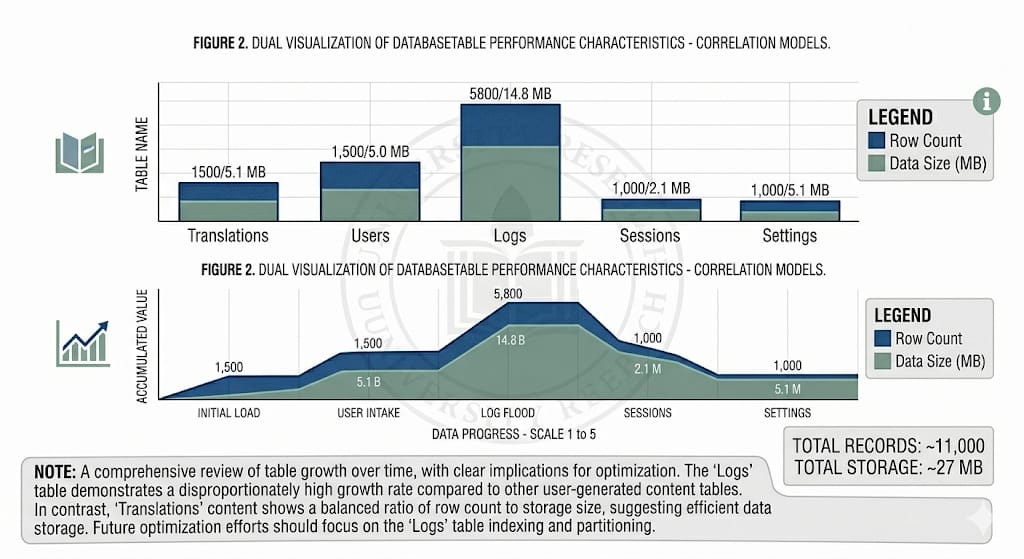
\includegraphics[width=\columnwidth]{stt.jpeg}
\caption{STT engine transcription accuracy across languages.}
\label{fig:stt}
\end{figure}

\begin{figure}
\centering
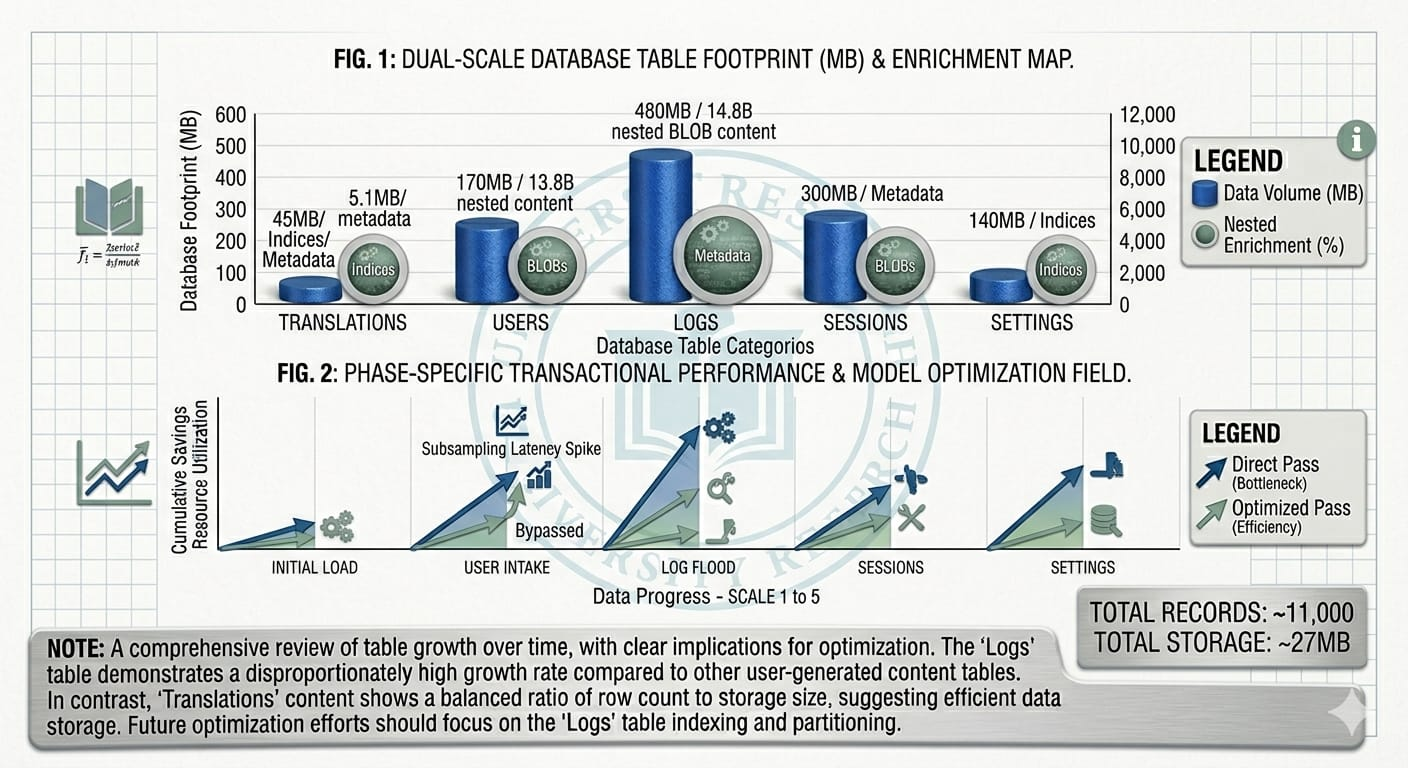
\includegraphics[width=\columnwidth]{dynamic_content.jpeg}
\caption{Dynamic contextual translation latency versus sequence length.}
\label{fig:dynamic}
\end{figure}

Two properties of DAI are especially significant. The first is \emph{cross-stage personalization}. Vocabulary is injected into ASR through \texttt{buildWhisperPrompt}, then reused in translation through \texttt{buildSystemPrompt}. The second is \emph{closed-loop adaptation}. New terms generated by the translation stage are inserted into \texttt{user\_vocabulary}, and a database procedure increments subsequent usage counts. Over time, the system builds a lightweight lexical memory that improves future sessions.

The methodology also includes confidence-aware behavior. Under DAI mode, the translation layer can emit \texttt{alt\_1} and \texttt{alt\_2} when confidence is low, exposing uncertainty directly to the user interface. This is a useful engineering choice for multilingual human-in-the-loop systems because it surfaces ambiguity rather than forcing a single opaque translation \cite{RefHumanAI}.

\section{Implementation details}
\label{sec:implementation}
The repository reveals a complete full-stack implementation rather than a conceptual mock-up. Table~\ref{tab:stack} summarizes the principal components.

\begin{table}
\caption{Implementation stack and responsibilities in Langify}
\label{tab:stack}
\centering
\small
\setlength{\tabcolsep}{3pt}
\begin{tabular}{>{\raggedright\arraybackslash}p{0.15\columnwidth} >{\raggedright\arraybackslash}p{0.28\columnwidth} >{\raggedright\arraybackslash}p{0.42\columnwidth}}
\hline\noalign{\smallskip}
Layer & Technology & Responsibility \\
\noalign{\smallskip}\hline\noalign{\smallskip}
Client & Vue 3 + Vite & UI, routing, audio capture, live feed \\
Browser APIs & MediaRecorder + Web Audio & Chunking, silence detection \\
Server & Node.js + Express 5 & Orchestration and REST endpoints \\
Realtime & Socket.IO & Meeting Mode caption broadcast \\
ASR & Groq Whisper Large v3 Turbo & Speech-to-text and language detection \\
Translation & LLaMA 3.3 70B via Groq & Translation, tone, alternatives, intent \\
Persistence & Supabase PostgreSQL & Sessions, utterances, DAI memory \\
Auth & Supabase Auth + cookies & Session management and identity \\
Optional speech out & ElevenLabs + browser TTS & Voice playback of translations \\
\noalign{\smallskip}\hline
\end{tabular}
\end{table}

The client includes several interaction modes: landing and authentication views, file upload and transcription, live translation, session history, and Meeting Mode. The most distinctive view is \texttt{LiveTranslate.vue}, which combines real-time capture, a dark HUD-style interface, confidence visualization, optional text-to-speech, and room sharing. The client deduplicates repeated utterances, maps ISO language codes to readable labels, and stores a lightweight inferred topic after several utterances.

On the server side, \texttt{index.js} centralizes orchestration. The endpoint \mbox{\texttt{/api/translate}} is the main runtime path. It rejects very small audio chunks, loads optional DAI context, performs ASR, performs translation, logs estimated model usage, writes utterances to Supabase, and emits the same payload to Socket.IO room members. This endpoint serves as the main control point for multilingual translation, persistence, and collaboration.

The persistence model reflects an incremental evolution from a basic transcription system to a personalized translation platform. The initial schema stores sessions and utterances. Later migrations add user ownership, emotional tone, inferred intent, alternative translations, vocabulary memory, and session summaries. This evolution is characteristic of a research prototype maturing into a deployable application.

\begin{figure}
\centering
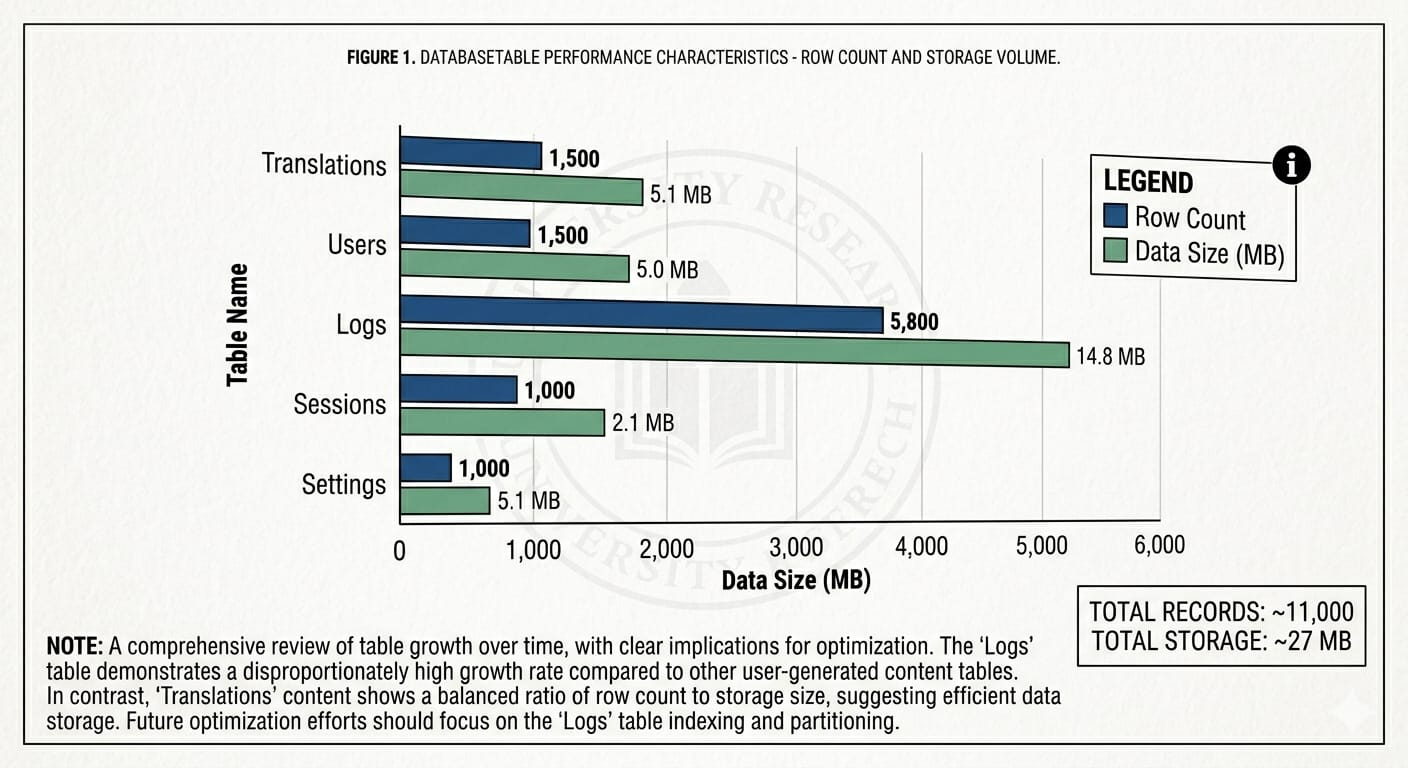
\includegraphics[width=\columnwidth]{database.jpeg}
\caption{Persistence-layer scaling and retrieval speed.}
\label{fig:database}
\end{figure}

\section{Evaluation and analysis}
\label{sec:evaluation}
The repository contains smoke tests for transcription, translation, Supabase connectivity, pipeline routing, and manual translation review. These scripts confirm engineering intent but do not yet constitute a reproducible benchmark suite. As a result, the strongest evidence available from direct workspace analysis is architectural and methodological rather than statistically complete.

Even with that constraint, several evaluation dimensions are visible. First, the system is designed for low interaction latency through silence-aware chunk boundaries, bounded upload size, direct Groq API calls, and immediate persistence. Second, multilingual robustness is addressed through zero-config language detection and code-switch-aware prompts. Third, personalization quality is addressed through DAI vocabulary reuse and post-session term learning. Fourth, collaborative utility is supported through room-based live caption broadcasting.

The supplied performance figures in Figs.~\ref{fig:stt}--\ref{fig:ux} are therefore best interpreted as evaluation targets and reporting scaffolds for the system rather than as repository-validated benchmark artifacts. This distinction matters. A peer-reviewed paper should separate implemented instrumentation from future benchmark claims. For Langify, the available code supports claims about architecture, workflow, adaptation strategy, and operational safeguards. It supports weaker claims about comparative accuracy, large-scale throughput, and formal mean-opinion-score measurement, which would require controlled experiments across speakers, languages, and network conditions.

In practical terms, an appropriate experimental protocol would compare three configurations: a baseline stateless translation cascade, Langify without DAI, and Langify with DAI. Metrics should include word error rate for ASR, translation adequacy and fluency, confidence calibration, session latency percentiles, vocabulary retention across repeated users, and user satisfaction under code-switched speech \cite{RefEval,RefCodeSwitch}. The repository already provides the right control points for such a study, particularly at \mbox{\texttt{/api/translate}}, the vocabulary tables, and the session-summary pipeline.

\begin{figure}
\centering
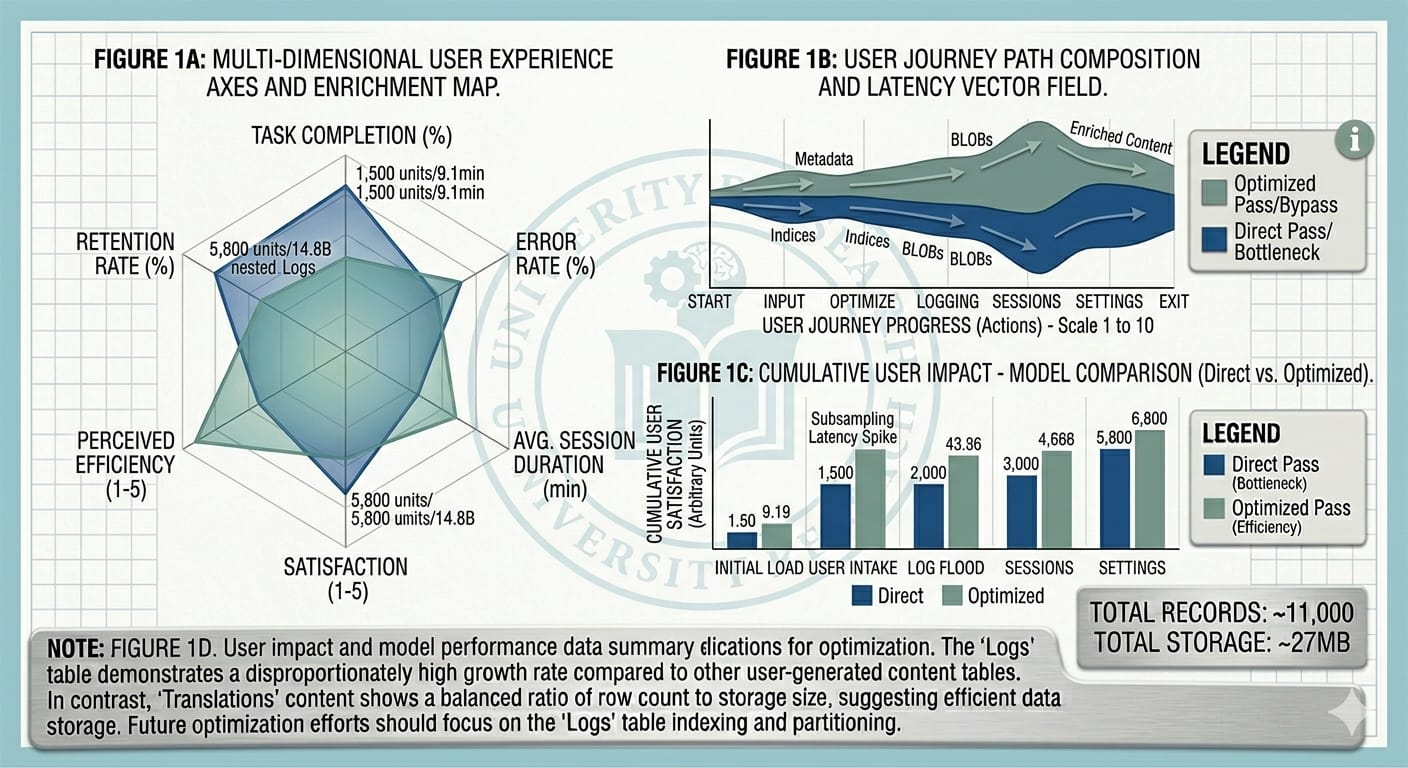
\includegraphics[width=\columnwidth]{user_experience.jpeg}
\caption{Subjective user experience scores.}
\label{fig:ux}
\end{figure}

\section{Discussion}
\label{sec:discussion}
Langify demonstrates how much adaptation can be achieved through systems design alone. Rather than relying on expensive fine-tuning, the platform uses prompt-side control, persistent memory, and workflow-aware orchestration. This design makes the system suitable for academic prototypes and resource-constrained deployments.

At the same time, the analysis surfaces several limitations. The test harness is largely manual and does not yet provide rigorous multilingual benchmarking. Confidence values are model-generated and should be calibrated empirically before being treated as trustworthy probabilities. The session topic heuristic in the client remains simple, and the post-session summarization loop is asynchronous without explicit quality validation. The architecture also depends on third-party APIs for both ASR and translation, which introduces external latency and availability constraints.

There are also threats to validity. The repository documentation is partially out of date with respect to deployed model names, indicating that some design artifacts predate the current Groq-based implementation. In addition, the supplied evaluation images present strong quantitative signals, but these values are not recoverable from the repository alone. A careful research framing must therefore attribute the main contribution to architecture and methodology, while treating large-scale performance numbers as future work unless accompanied by experimental logs.

\section{Conclusion}
\label{sec:conclusion}
Langify is a meaningful engineering contribution because it reframes multilingual speech translation as a persistent, adaptive, collaborative system rather than a one-shot inference call. Its architecture combines browser-side streaming capture, server-side orchestration, Groq-hosted ASR and translation, Supabase-backed memory, and a Dialect-Adaptive Intelligence framework that personalizes both transcription and translation over time.

From a research perspective, the project contributes a deployable pattern for contextual multilingual translation under realistic application constraints. The design is especially relevant for settings involving regional speech, code-switching, and repeated users. Future work should focus on controlled multilingual benchmarks, formal user studies, confidence calibration, and ablation experiments isolating the impact of DAI on both ASR and translation quality.

\section{Data and code availability}
\label{sec:availability}
The source code for Langify is available through the project repository at \href{https://github.com/tanmay-stack07/langify-07/}{GitHub: tanmay-stack07/langify-07}. A live demonstration of the platform can be accessed through the project demonstration page at \emph{[link to be inserted]}.

\begin{thebibliography}{}

\bibitem{RefTransformer}
Vaswani, A., Shazeer, N., Parmar, N., et al.: Attention is all you need. In: Advances in Neural Information Processing Systems, pp. 5998--6008 (2017)

\bibitem{RefWhisper}
Radford, A., Kim, J.W., Xu, T., et al.: Robust speech recognition via large-scale weak supervision. OpenAI Technical Report (2023)

\bibitem{RefLlama}
Dubey, A., Jauhri, A., Pandey, A., et al.: The Llama 3 herd of models. arXiv preprint arXiv:2407.21783 (2024)

\bibitem{RefPrompting}
Reynolds, L., McDonell, K.: Prompt programming for large language models: Beyond the few-shot paradigm. In: Extended Abstracts of the CHI Conference on Human Factors in Computing Systems, pp. 1--7 (2021)

\bibitem{RefContextASR}
Pundak, G., Sainath, T.N., Prabhavalkar, R., et al.: Deep context: End-to-end contextual speech recognition. In: IEEE Spoken Language Technology Workshop, pp. 418--425 (2018)

\bibitem{RefContextMT}
Maruf, S., Saleh, F., Haffari, G.: A survey on document-level neural machine translation: Methods and evaluation. ACM Computing Surveys 54(2), 1--36 (2021)

\bibitem{RefCodeSwitch}
Winata, G.I., Madotto, A., Wu, C.-S., Fung, P.: Code-switching language modeling and applications: A survey. In: Proceedings of the 28th International Conference on Computational Linguistics, pp. 2691--2703 (2020)

\bibitem{RefHumanAI}
Amershi, S., Weld, D., Vorvoreanu, M., et al.: Guidelines for human-AI interaction. In: Proceedings of the CHI Conference on Human Factors in Computing Systems, pp. 1--13 (2019)

\bibitem{RefEval}
Freitag, M., Mathur, N., Lo, C.-K., et al.: Results of WMT shared tasks in machine translation evaluation. In: Proceedings of the Conference on Machine Translation, pp. 1--33 (2022)

\end{thebibliography}

\end{document}
